%%中山大学物理学院-基础物理实验-论文格式报告模板1.1
%%完成整理日期:2020/2/18
%%更新时间:2020/8/25
%%中山大学物理学院18级 王佛泓
%%文本编辑器:Sublime Text
%%平台:win10, Texlive 2019

%---------------------导言区---------------------------%
\documentclass[10pt,a4paper,twocolumn,twoside,UTF8]{ctexart}
	%10pt:正文字体为10pt,可以缺省;各层级字体大小会根据正文字体自动调整
	%a4paper:纸张大小a4;
	%twocolumn:双栏排版;
	%twoside:排版上分奇偶页,一般也就是有双面打印的需求;
	%UTF8:中文要求
\usepackage{geometry}%用于设置上下左右页边距
	%左右边距一样: 不考虑装订和翻页的需要.实验室网站上的示例论文格式报告就是这样。
	\geometry{left=2cm,right=2cm,top=2.5cm,bottom=4cm}
	%实际上,一般需要考虑到双面打印、装订和翻页的需要,需要区分奇偶页。奇偶页的页边距需要分开设置。奇数页左边距较宽,偶数页左边距较窄。
\usepackage{xeCJK,amsmath,paralist,enumerate,booktabs,multirow,graphicx,float,subfig,setspace,listings}
	%xeCJK:中文字体(如楷体,作者和机构需要用到)的设置
	%amsmath:数学公式
	%paralist,enumerate:自定义项目符号
	%booktabs:三线图,论文常用的表格风格
	%multirow:复杂表格
	%graphicx,float: 插入图片
	%subfig:并排排版图片以及强制图表显示在“这里”[H]
	%setspace:设置行间距等功能
	\setlength{\parindent}{2em}%正文首行缩进两个汉字
	%listings:用于排版各种代码;比如matlab的代码
	\lstset{language=Matlab}%matlab代码
	%代码环境的使用可以参考完整实验报告模板

\setCJKmainfont{FZShuSong-Z01S}[ItalicFont=FZKai-Z03S, BoldFont=FZHei-B01S]
%中文字体设置:使用开源字体方正书宋,方正楷体和方正黑体

\usepackage{titlesec}
	%改变section、subsection里面字体的样式。中文黑体,英文TNR。
	\newfontfamily\sectionef{Times New Roman}
	\setCJKfamilyfont{FZHeiTi}{FZHei-B01S}
	\newcommand{\sectioncf}{\CJKfamily{FZHeiTi}}
	\titleformat*{\section}{\large\bfseries\sectioncf\sectionef}
	\titleformat*{\subsection}{\normalsize\bfseries\sectioncf\sectionef}	


\usepackage{fancyhdr}
	%fancyhdr:一个很强大的宏包,用于自定义设计页面风格并命名以供调用。



%%begin----------设置首页和正文不同的页眉页脚----------------%%

\usepackage{ifthen}%这个宏包提供逻辑判断命令
\newboolean{first}%引入布尔变量
\setboolean{first}{true}%将布尔变量设置为true
\pagestyle{fancy}

	%%% Step1 定义正文的页面风格
	%E表示偶数页,O表示奇数页;R、L、C代表文字居右、居左、居中排版
	%页码:保证在外侧, 奇数页分布在右边,偶数页分布在左边
	%页眉中间的内容也因奇偶页而不同
	%实验名称根据实际情况修改
	\fancypagestyle{maincontent}{  
		\fancyhf{}  %清空页眉页脚设置
		\fancyhead[EL, OR]{\thepage}
		\fancyhead[EC]{实验B12 温度测控仪的设计与组装}
		\fancyhead[OC]{基\quad 础\quad 物\quad 理\quad 实\quad 验}
		\renewcommand\headrulewidth{0pt}
	}

	%%% Step2 定义首页的页面风格
	%页眉中间的双行文字,大小和字间距需要微调
	%左右的内容是年月,可以自己修改寻找自动获取的方法
	\usepackage{datetime}
		%\shortmonthname可以获取英文月份缩写
	\fancypagestyle{firstpage}{
		\setboolean{first}{false}%firstpage出现,则将first重置为false
		\fancyhf{}  %清空页眉页脚设置
		\fancyhead[L]{\the\year 年\the\month 月}
		\fancyhead[R]{\shortmonthname[\the\month], \the\year}
		\fancyhead[C]{
		          \large{基\quad 础\quad 物\quad 理\quad 实\quad 验}\\ 
		          \normalsize{GENERAL PHYSICS LABORATORY}
		          }
	}

	%%% Step3 页眉线的设置:用布尔变量区分首页和正文
	\newcommand{\makefirstpageheadrule}{%定义首页页眉线-双线绘制命令
		\makebox[0pt][l]{\rule[0.55\baselineskip]{\headwidth}{0.2pt}}%上0.5pt,下0.2pt
		\rule[0.7\baselineskip]{\headwidth}{0.5pt}
	}

	\newcommand{\makeheadrule}{%定义正文页页眉线绘制命令,单线
		\rule[0.7\baselineskip]{\headwidth}{0.75pt}
	}

	%根据布尔变量first为true或false分别执行不同的页眉线绘制命令
	\renewcommand{\headrule}{%重定义headrule命令
		\ifthenelse{\boolean{first}}{\makeheadrule}
		{\makefirstpageheadrule}
	}



%%end--------------设置首页和正文不同的页眉页脚-----------%%



%%begin-----------------参考文献-----------------------%%

\usepackage{hyperref}%超链接
\usepackage[hyperref=true,backend=biber,bibstyle=gb7714-2015,citestyle=numeric-comp,sorting=none,backref=true]{biblatex}
	%hyperref=true和backref=true表示为各个参考文献的引用处、及定理、定义、例子等的引用处都添加上超链接;
	%backend=biber:后端处理的程序为biber.exe
	%bibstyle:参考文献风格;每个期刊、组织要求不同
		%gb7714-2015是目前国内期刊通用的风格,称为gb标准风格
	%citestyle:引用风格;每个期刊、组织要求不同
	%sorting=none:按照参考文献在论文中出现的先后顺序排序。
	%**编译:biblatex与biber命令配合使用。xelatex-biber-xelatex-xelatex
\addbibresource{book.bib}
	%这里写上.bib文件的相对地址
	%每次实验引用的页数不同,需要手动改变

%%end-------------------参考文献-----------------------%%



\setCJKfamilyfont{fzyao}{FZYaoTi}                                    %方正姚体  fzy
\newcommand{\fzyao}{\CJKfamily{fzyao}}



%%%%%%%%%%%%%%%%%%%%%%%%%%%%%%%%%%%%%%%%%%%%%%%%%%%%%%%%%%
%%%%%%%%%%%%%%%%%%%%%%%%%正文开始%%%%%%%%%%%%%%%%%%%%%%%%%%
%%%%%%%%%%%%%%%%%%%%%%%%%%%%%%%%%%%%%%%%%%%%%%%%%%%%%%%%%%

\begin{document}


%%begin-------------------中文摘要-----------------------%%
\title{\LARGE\textbf{实验B12 温度测控仪的设计与组装}}
\author{\large\textit{鸭大学子}$^{1}$\\ \normalsize{(1 \textit{中山大学 物理学院,广东 广州 }510275)}}
\date{}%不显示日期

\twocolumn[
	%twocolumn: 双栏article下的单栏摘要
	\begin{@twocolumnfalse}
	\maketitle  %标题和作者
  	\renewcommand{\abstractname} {} %不显示摘要名字
	\begin{abstract}
	\vspace{-3em} 
	%vspace:调整垂直空白,可以自己调整;缩小abstract和center(以及maketitle)的间距
	%\noindent %备用:摘要无缩进
	{\bf 摘{} 要:}
	{\small 温度传感器是利用一些金属、半导体等材料与温度相关的特性制成的。温度传感器的类型很多,包括金属电阻温度传感器、热敏电阻温度传感器、热电偶温度传感器、PN结温度传感器、电压型集成电路温度传感器和电流型集成电路温度传感器等等。本实验通过搭建基于电压型集成电路温度传感器的温度测控电路,学习了温度传感器测量和控制温度的基本原理,并测试了搭建的测控电路的有效性。}
	\par%空的新行的高度。
	\textbf{关键词}:温度传感器; LM35
	\vspace{2em}
	\end{abstract}
	\end{@twocolumnfalse}
]	

%%end-------------------中文摘要-----------------------%%

\thispagestyle{firstpage}%首页页面风格:firstpage
\pagestyle{maincontent}%第二页之后的页面风格:maincontent

%%begin----------------层级结构------------------------%%

%重点1:知道每一个层级的样式和怎么和后面的正文接上
%重点2:掌握各种换段的方法
%重点3:自定义的项目符号(宏包enumerate的用法)

\section{引 \quad 言}
	%%section:第一级,节	,1
在大一的实验 A4(温度传感器温度特性的测量)\cite{shenhan2015}中已经了解了多种温度传感器的特性和工作原理,本实验将在此基础上,利用温度传感器,设计并组装数字式温度计和温度控制仪。
	%%section后面的正文:自动换段,正常缩进
	%%PS:这里出现了引用。一般就是做个样子,在引言引一下参考文献就好了。不引用后面的参考文献打印不出来。
由于这一实验的巨大成就,密立根获得了1923年的诺贝尔物理学奖。\par
	%%自然换段:\par
80多年来,显示出该实验在工业应用和科学研究中的广泛应用前景。\par
笔者利用大学实验室常用的密立根油滴实验仪重做了密立根油滴实验,并尝试由实验结果验证电荷分布的不连续性,将在本文中详述。

\newpage
%换一栏,而不是换一页。换一页用\clearpage
\section{温度测控原理}
温度的测控,包含温度的测量和控制,其中温度的测量往往转化为电信号输出,而温度的控制通常使用电磁继电器实现。本实验设计的温度测控仪器主要包括两个部分,一个是温度传感器,另一个是温度测控电路。

	\subsection{温度测控仪电路}
		%%subsection:第二级,小节,2.1
	基于以上三种温度测控仪,我们相应得也有三种温度测控仪电路。
		%%subsection后面的正文:自动换段,正常缩进
	\subsubsection{基于 AD590 电流型温度传感器的数显温度测控仪}
		%%subsubsection: 第三级,小小节,2.1.1
	这里本来并不需要文字。
		%%subsubsection后面的正文:自动换段,正常缩进
	\paragraph{A.温度显示原理}
		%%paragraph: 大段落,加粗,不缩进
	如果就需要这样的效果,那很好。
	\paragraph{B.温度控制原理}但段落后面如果需要换行,就是个棘手的问题。
		%%paragraph后面的正文:无论是紧接着}敲还是换了几行,都会空一到两格后直接跟在后面。
	\subparagraph{第一步:调零。}小段落后面的正文也是一样,
		%%subparagraph:小段落,加粗,正常缩进
	\subparagraph{第二步:确定电压灵敏度}
	紧跟着段落标题。
		%%subparagraph后面的正文:无论是紧接着}敲还是换了几行,都会空一到两格后直接跟在后面。


	\subsection{温度传感器}
	本实验涉及三种温度测控仪的组装,分别采用三种不同的温度传感器,包括
	%%paragraph后面的换段方法
	\paragraph{(1)金属电阻温度传感器}~
		% ~是一个控制符号,不会真的输出~,而是空一格。
	\newline %换行,强制换行之后需要手动缩进,用命令\indent
	\indent 如 PT100 或 Cu50, PT100 即铂金属电阻,在 0℃时的电阻值为 $R_0=100\Omega$; Cu50 即铜金属电阻, 在 0℃时的电阻值为$R_0=50\Omega$。


	\subsection{实验内容}
	本实验中笔者选择了“基于LM35电压型温度传感器的数显温度测控仪”电路进行搭建和测试。
	%%自定义项目符号之(1)(2)(3)
	\begin{enumerate}[(1)] 
		\item 根据图5搭建电路。
		\item 测量数字电压读数与温度之间的对应关系, 作电压与温度关系曲线。
	 	\item 利用组装的温度测控仪电路,将加热阱的温度控制在 75$^{\circ}C$。
	\end{enumerate}

%%end------------------层级结构------------------------%%

%%begin------------------插入图表------------------------%%

\section{温度测控仪的搭建和测试}
	
	\subsection{测试用设备}
	\paragraph{A.其他设备}~
	\newline
	\indent 直流稳压电源用于提供测控仪电路的±12V电源,数字万用表的直流电压测量功能可用于替代数字电压表,用于指示温度测控仪的当前温度。各仪器使用方法请查阅教材。

%%% 1 不跨栏单幅图
	% 图片的大小需要细细得调。需要掌握latex里面的长度单位和限制大小方法。
	\begin{figure}[htbp]
		\centering
		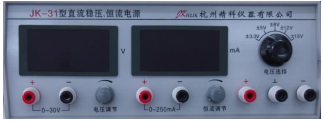
\includegraphics[width=0.5\textwidth]{img//device_3.png}
			%textwidth:正文宽度。双栏,则将两栏正文宽度相加。
		\caption{直流稳压电源}
		\label{powersource}
	\end{figure}

%%% 2 跨栏单幅图
	% 在figure之右加上*即可。
	\begin{figure*}[htbp]
	\centering
	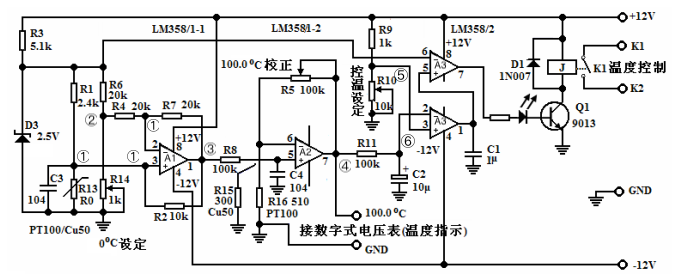
\includegraphics[width=1\textwidth]{img//Diagram_Cu50.png}
	\caption{基于 PT100(或 Cu50)温度传感器的数显温度测控仪}
	\label{Diagram_Cu50}
	\end{figure*}
	
	\paragraph{B.温度控制设备}~
	\newline

%%% 3 两幅图并行排版,各有图题,还有一个总的图题
	% (1)注意正文中引用图片的方法
	% (2)不仅需要调节大小,还需要细细调节位置。通过{minipage}后面的补充参数来调节位置。图片大小最好用高度来调,并保证两个图高度一样。
	\indent 图\ref{fig:improved_subfig_a}为致冷/加热温度控制仪,从左到右分成三个部分,分别为(1)数字电压表(有20V和2V两个量程);(2)加热和致冷功率控制器;(3)温度设置和测量装置风扇用于加快空气流动。
	图\ref{fig:improved_subfig_b}的控温阱分为致冷阱和加热阱两种。制冷阱用于0℃至室温范围的实验,加热阱用于室温-100℃范围。

	\begin{figure*}[htbp]
		\centering
		\subfloat[致冷/加热温度控制仪]{
		\label{fig:improved_subfig_a}
		\begin{minipage}{0.5\textwidth}
			\centering
			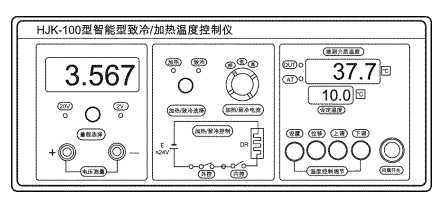
\includegraphics[height=5cm]{img//device_1.png}
		\end{minipage}
		}
		\subfloat[控温阱]{
		\label{fig:improved_subfig_b}
		\begin{minipage}{0.5\textwidth}
			\centering
			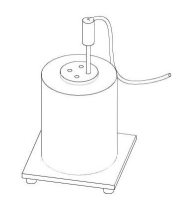
\includegraphics[height=5cm]{img//device_2.png}
		\end{minipage}
		}
		\caption{温度控制设备}
	\end{figure*}
	
\section{实验结果与讨论}

	\subsection{数字电压读数与温度的对应关系}
	将测控电路接入加热阱,记录温度传感器温度为$30^{\circ}C到80^{\circ}C$对应的数字电压表示数。分别记录温度上升时和温度下降时的电压值,取平均以降低误差,如表\ref{tab:addlabel}所示。

%%% 4 不跨栏表格
	%所有表格都可以通过Excel2LaTex加载项,在excel中转换成以下一串代码。需要琢磨的是调节一些细节的方法。

	% Table generated by Excel2LaTeX from sheet 'Sheet1'
	\begin{table}[htbp]
	  \centering
	    \begin{tabular}{cccc}
	    \toprule
	    t/$^{\circ}$C & 上升/mV & 下降/mV & 平均$V_0/mV$ \\
	    \midrule
	    30    & 271   & 280   & 275.5 \\
	    32.9  & 299   & 313   & 306 \\
	    37.8  & 336   & 363   & 349.5 \\
	    40.9  & 364   & 396   & 380 \\
	    42.7  & 387   & 414   & 400.5 \\
	    45    & 414   & 438   & 426 \\
	    50    & 460   & 489   & 474.5 \\
	    53    & 475   & 518   & 496.5 \\
	    55    & 494   & 538   & 516 \\
	    58    & 522   & 568   & 545 \\
	    60    & 540   & 588   & 564 \\
	    63    & 569   & 617   & 593 \\
	    65    & 589   & 636   & 612.5 \\
	    70    & 639   & 684   & 661.5 \\
	    73    & 669   & 711   & 690 \\
	    75    & 690   & 729   & 709.5 \\
	    78    & 721   & 753   & 737 \\
	    80    & 748   & 768   & 758 \\
	    \bottomrule
	    \end{tabular}%
	  \caption{数据记录}
	  \label{tab:addlabel}%
	\end{table}%

%%% 5 跨栏表格
	%手动在table右边加上*即可

	% Table generated by Excel2LaTeX from sheet '打印'
	\begin{table*}[htbp]
	  \centering

	    \begin{tabular}{c|ccccc}
	    \toprule
	    \multicolumn{1}{c}{} & 油滴序号  & Q/C   & Q/e   & n     & e/C \\
	    \midrule
	    \multicolumn{1}{c}{\multirow{5}[2]{*}{静态法}} & 1     & 1.713E-19 & 1.069  & 1     & 1.713E-19 \\
	    \multicolumn{1}{c}{} & 2     & 5.681E-19 & 3.546  & 4     & 1.420E-19 \\
	    \multicolumn{1}{c}{} & 3     & 5.710E-19 & 3.564  & 4     & 1.428E-19 \\
	    \multicolumn{1}{c}{} & 4     & 1.292E-18 & 8.062  & 8     & 1.615E-19 \\
	    \multicolumn{1}{c}{} & 5     & 9.490E-19 & 5.923  & 6     & 1.582E-19 \\
	    \midrule
	    \multicolumn{1}{c}{} &       & 平均值:  & 1.551E-19 & 相对误差: & 3.169\% \\
	    \midrule
	    \multicolumn{1}{c}{\multirow{5}[2]{*}{动态法}} & 6     & 1.253E-18 & 7.821  & 8     & 1.566E-19 \\
	    \multicolumn{1}{c}{} & 7     & 3.174E-19 & 1.981  & 2     & 1.587E-19 \\
	    \multicolumn{1}{c}{} & 8     & 1.234E-18 & 7.701  & 8     & 1.542E-19 \\
	    \multicolumn{1}{c}{} & 9     & 9.402E-19 & 5.868  & 6     & 1.567E-19 \\
	    \multicolumn{1}{c}{} & 10    & 6.309E-19 & 3.938  & 4     & 1.577E-19 \\
	    \midrule
	    \multicolumn{1}{c}{} &       & 平均值:  & 1.568E-19 & 相对误差: & 2.133\% \\
	    \multicolumn{2}{c}{整体情况} & 平均值:  & 1.560E-19 & 相对误差: & 2.651\% \\
	    \bottomrule
	    \end{tabular}%
	 \caption{数据处理}
	\end{table*}%


%%end--------------------插入图表------------------------%%


%%begin------------------插入公式------------------------%%

\section{结论}
美国物理学家密立根(Robert a. Millikan)在$1909 \sim 1917$年期间所做的测量微小油滴上所带电荷的工作,即油滴实验,是物理学发展史上一个具有重要意义的实验。这一实验的设计思想简明巧妙、原理清楚、设备简单、结果准确。本实验通过重做密立根的油滴实验,通过“倒过来验证”的方法从实验上验证了电荷分布的不连续性。采用的仪器是专用的密立根油滴实验仪,操作更加方便和清晰。

	1 需要标号、单个公式
		%一般来说都需要标号
		\begin{equation}
		\eta^{\prime}=\eta /[1+b /(p a)]
		\end{equation}

	2 需要标号、多个公式、不需要对齐
		\begin{gather}
		f_r=6\pi a \eta v_g   \\
		m=4 \pi a^{3} \rho / 3
		\end{gather}

	3 需要标号、多个公式、需要对齐		
		\begin{align}
		a &= b+c+d \\
		x &= y+z
		\end{align}

	4 不需要标号,单个公式
		\[e=(1.60217733 \pm 0.00000049) \times 10^{-19} \mathrm{C}\]
		另一种方法:
		\begin{equation*}
		e=(1.60217733 \pm 0.00000049) \times 10^{-19} \mathrm{C}
		\end{equation*}

	5 不需要标号,多个公式,不需要对齐/需要对齐
		%使用对应的*版本
		\begin{gather*}
		f_r=6\pi a \eta v_g   \\
		m=4 \pi a^{3} \rho / 3
		\end{gather*}
		另一种方法:
		\begin{align*}
		a &= b+c+d \\
		x &= y+z
		\end{align*}

	6 长公式,换行,不对齐
		%不标号的话加上*
		\begin{multline}
		x = a+b+c+{} \\
		d+e+f+g
		\end{multline}

	7 长公式,换行,对齐
		%aligned:次环境
		\[\begin{aligned}
		x ={}&a+b+c+{} \\
		&d+e+f+g
		\end{aligned}\]

	8 带有左边大括号的公式
	\[\left\{
		\begin{aligned}
		&C_{1} \cdot \frac{d U_{C_{1}}}{d t}=\frac{1}{R_{1}} \cdot(u_{C_{2}}-u_{C_{1}})-f(u_{R_{N}}) \\
		&C_{2} \cdot \frac{d U_{C_{2}}}{d t}=i_{L}-\frac{1}{R_{1}} \cdot(u_{C_{2}}-u_{C_{1}}) \\
		&L \cdot \frac{d i_{L}}{d t}=-U_{C_{2}}
		\end{aligned}
	   \right.
	\]

%%end--------------------插入公式------------------------%%

\printbibliography[title=参考文献]%打印参考文献
	%title:默认是英文的reference,用这个选参数改成中文



%%begin------------------英文摘要------------------------%%

\twocolumn[
\begin{@twocolumnfalse}
	\renewcommand{\abstractname} {} %不显示摘要名字
	\begin{center}%
	    {\LARGE\bfseries Experiment B12: The Design and Assembling of Temperature Sensor \par}%
	    \vskip 1.4em%
	    {\large
	     \lineskip .75em%
	      \begin{tabular}[t]{c}%
	        \large Fohong Wang$^{1}$
	      \end{tabular}\par
	      }%
	      \vskip 0.4em%
	    {\normalsize 1 School of Physics, Sun Yat-sen University, Guangzhou  { \rm 510275}, China}
	\end{center}
	\begin{abstract}  
		\vspace{-2em}  %缩小abstract和center(以及maketitle)的间距
	    	{\bf Abstract:}  
	     {\small The temperature sensor is made of some metal, semiconductor and other materials with temperature-related characteristics. There are many types of temperature sensors, including metal resistance temperature sentors, thermistor temperature sensors, voltage-type integrated circuit temperature sensors and current-type integrated circuit temperature sensors. In this experiment, by building a temperature measurement and control circuit based on a voltage-type integrated circuit temperature sensor, the basic principles of temperature sensor measurement and control were learned, and the effectiveness of the measurement and control circuit was tested.}
	  	\par%空的新行的高度。
		\textbf{Key words}:Temperature sensor, LM35
	\end{abstract}   
\end{@twocolumnfalse}
]
%%end--------------------英文摘要------------------------%%

\end{document}